
An activity diagram describes the control flow from a start point to a finish point showing the various decision paths that exist while the activity is being executed.The activity diagram for Kitab is categorized based on the Actor.


\begin{figure}[H]
\begin{center}	

	\tcbox{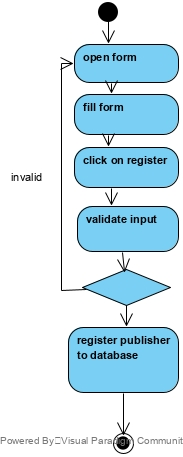
\includegraphics[width=0.4\textwidth]{Diagram/activity/Add Publisher.png}}
	\caption{Activity diagram for adding publisher.}
	\label{dia_actvt_addpblshr}

\end{center}
\end{figure}

\begin{figure}[H]
\begin{center}	

	\tcbox{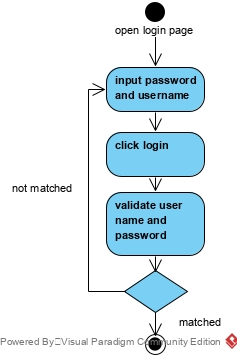
\includegraphics[width=0.6\textwidth]{Diagram/activity/Login.png}}
	\caption{Activity diagram for login.}
	\label{dia_actvt_login}

\end{center}
\end{figure}

\begin{figure}[H]
\begin{center}	

	\tcbox{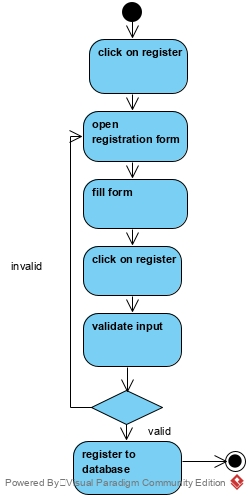
\includegraphics[width=0.6\textwidth]{Diagram/activity/Register.png}}
	\caption{Activity diagram for registering.}
	\label{dia_actvt_rgstr}

\end{center}
\end{figure}

\begin{figure}[H]
\begin{center}	

	\tcbox{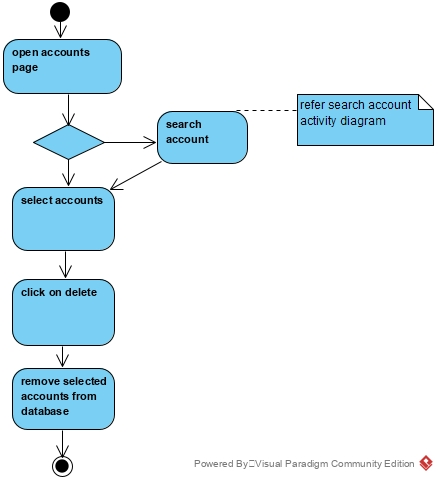
\includegraphics[width=0.6\textwidth]{Diagram/activity/Remove Account.png}}
	\caption{Activity diagram for removing account.}
	\label{dia_actvt_rmvaccnt}

\end{center}
\end{figure}

\begin{figure}[H]
\begin{center}	

	\tcbox{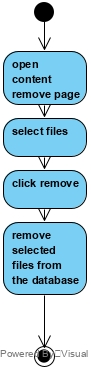
\includegraphics[width=0.2\textwidth]{Diagram/activity/Remove Content.png}}
	\caption{Activity diagram for removing content.}
	\label{dia_actvt_rmvcntnt}

\end{center}
\end{figure}

\begin{figure}[H]
\begin{center}	

	\tcbox{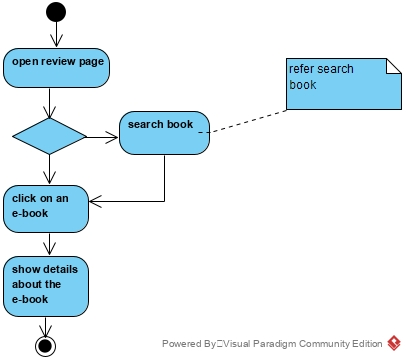
\includegraphics[width=0.6\textwidth]{Diagram/activity/Review.png}}
	\caption{Activity diagram for reviewing.}
	\label{dia_actvt_rvw}

\end{center}
\end{figure}

\begin{figure}[H]
\begin{center}	

	\tcbox{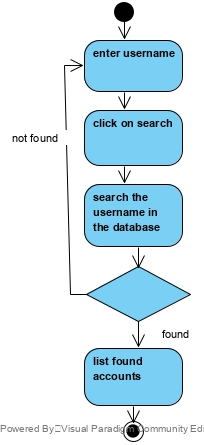
\includegraphics[width=0.4\textwidth]{Diagram/activity/Search Account.png}}
	\caption{Activity diagram for searching account.}
	\label{dia_actvt_srchaccnt}

\end{center}
\end{figure}

\begin{figure}[H]
\begin{center}	

	\tcbox{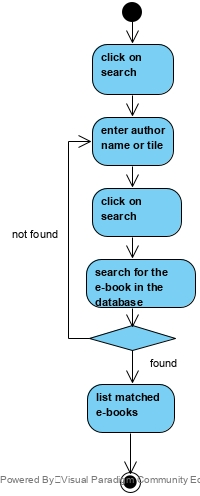
\includegraphics[width=0.4\textwidth]{Diagram/activity/Search Content.png}}
	\caption{Activity diagram for searching content.}
	\label{dia_actvt_srchcntnt}

\end{center}
\end{figure}

\begin{figure}[H]
\begin{center}	

	\tcbox{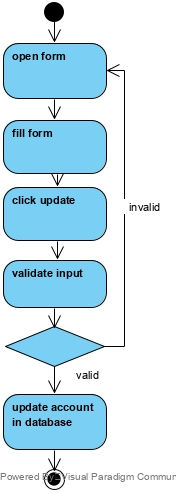
\includegraphics[width=0.4\textwidth]{Diagram/activity/Update Account.png}}
	\caption{Activity diagram for updating account.}
	\label{dia_actvt_updtaccnt}

\end{center}
\end{figure}

\begin{figure}[H]
\begin{center}	

	\tcbox{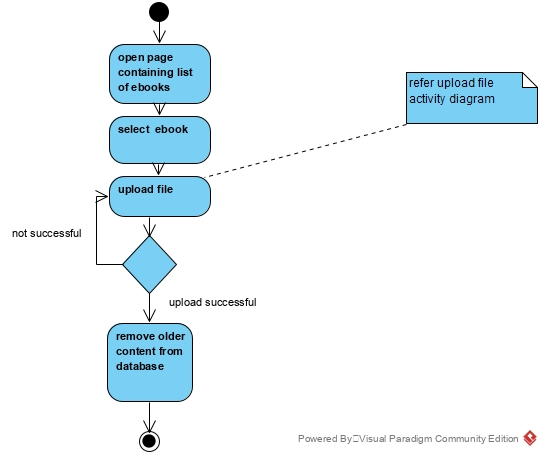
\includegraphics[width=0.6\textwidth]{Diagram/activity/Update Content.png}}
	\caption{Activity diagram for updating content.}
	\label{dia_actvt_updtcntnt}

\end{center}
\end{figure}

\begin{figure}[H]
\begin{center}	

	\tcbox{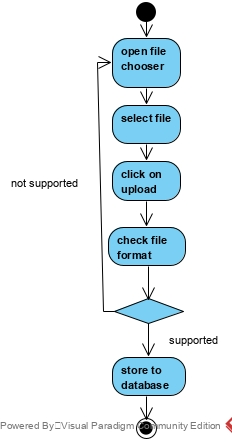
\includegraphics[width=0.6\textwidth]{Diagram/activity/Upload File.png}}
	\caption{Activity diagram for uploading file.}
	\label{dia_actvt_upldfl}

\end{center}
\end{figure}

\begin{figure}[H]
\begin{center}	

	\tcbox{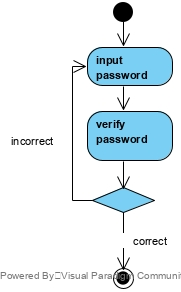
\includegraphics[width=0.6\textwidth]{Diagram/activity/Verify Password.png}}
	\caption{Activity diagram for verifying password.}
	\label{dia_actvt_vrfypsswd}

\end{center}
\end{figure}

\begin{figure}[H]
\begin{center}	

	\tcbox{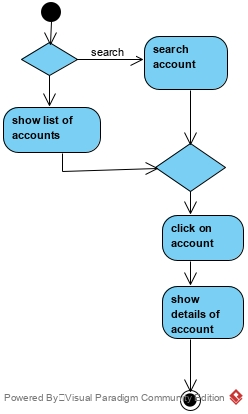
\includegraphics[width=0.6\textwidth]{Diagram/activity/View Account-details.png}}
	\caption{Activity diagram for viewing account details.}
	\label{dia_actvt_vwaccntdtls}

\end{center}
\end{figure}



































\begin{figure}[H]
\begin{center}	

	\tcbox{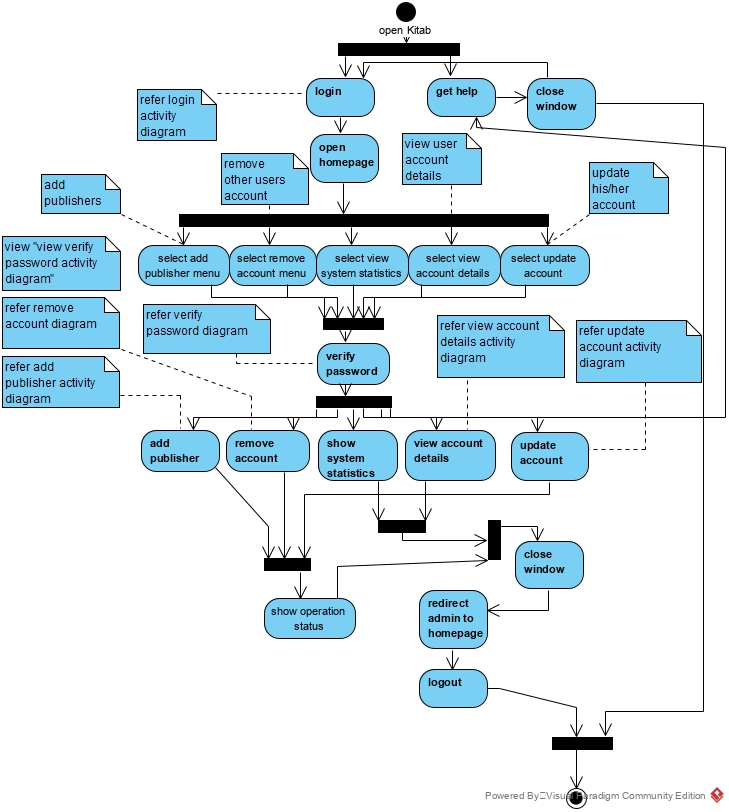
\includegraphics[width=\textwidth]{Diagram/activity/For Admin.png}}
	\caption{Activity diagram for admin.}
	\label{dia_actvt_fradmn}

\end{center}
\end{figure}

\begin{figure}[H]
\begin{center}	

	\tcbox{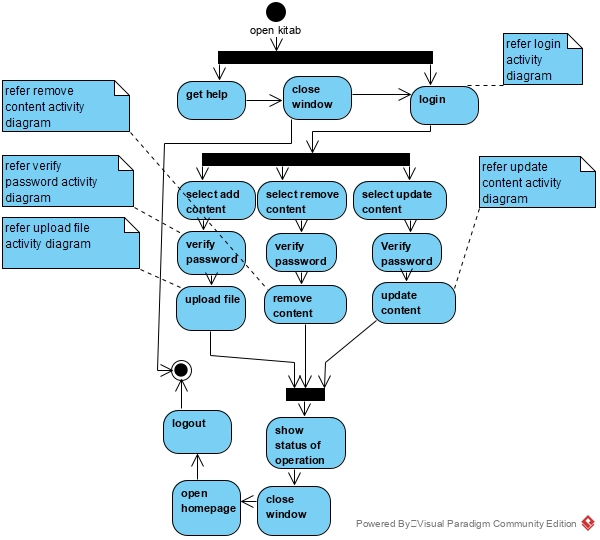
\includegraphics[width=\textwidth]{Diagram/activity/For Publisher.png}}
	\caption{Activity diagram for publisher.}
	\label{dia_actvt_frpblshr}

\end{center}
\end{figure}

\begin{figure}[H]
\begin{center}	

	\tcbox{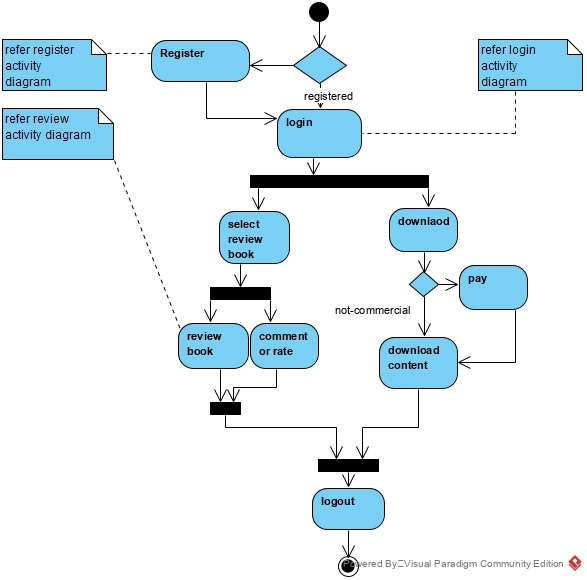
\includegraphics[width=\textwidth]{Diagram/activity/For Reader.png}}
	\caption{Activity diagram for reader.}
	\label{dia_actvt_frrdr}

\end{center}
\end{figure}
